\section{Evaluation Data}
\label{app:eval}

We compare how many instances the solvers handle within
1s, within 1-10s, 10-100s, and 10-600s. We also list
timeouts and cases where the solver returns unknown because of incompleteness,
and cases where benchmarks are unhandled, either because the solver runs out of allocated virtual memory set to 2GB,
or due to unsupported features. The version of Z3 used for the experiments correponds to 4.12.5.


\begin{table}
  \begin{tabular}{|l|c|c|c|c|c|c|c|}
    \hline
    Solver & $<$ 1s & 1 to 10s & 10 to 100s & 100 to 600s & $>$ 600s & unknown/unhandled & solved \\
    \hline
    CVC5 & 3082 & 4564 & 3578 & 1693 & 10959 & 0/0 & 12917 \\
    \hline
    MathSat5 & 3304 & 6022 & 3894 & 2047 & 8607 & 0/2 & 15267 \\
    \hline
    Yices2 & 6372 & 6284 & 2176 & 852 & 8192 & 0/0 & 15684 \\
    \hline
    z3 & 4597 & 7440 & 4826 & 1504 & 5505 & 0/4 & 18367 \\
    \hline
    z3legacy & 3504 & 6881 & 4081 & 1577 & 6923 & 891/19 & 16043 \\
    \hline
    \end{tabular}
  \caption{Comparison among solvers on QF\_NIA \label{tab:compare-qf-nia}}
\end{table}

\begin{figure}[htbp]
  \centering
  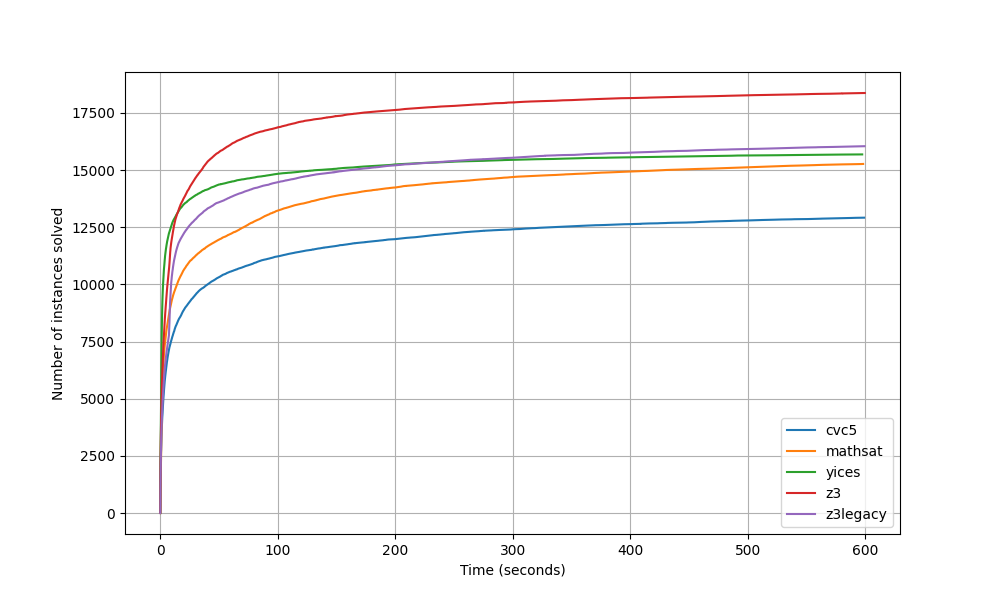
\includegraphics[width=0.99\textwidth]{..\data\compare-qf-nia.png}
  \caption{Compare solvers on QF-NIA }
  \label{fig:organization}
\end{figure}

\begin{table}
  \begin{tabular}{|l|c|c|c|c|c|c|c|}
    \hline
    Solver & $<$ 1s & 1 to 10s & 10 to 100s & 100 to 600s & $>$ 600s & unknown/unhandled & solved \\
    \hline
    CVC5 & 1540 & 1071 & 529 & 416 & 3391 & 0/0 & 3556 \\
    \hline
    MathSat5 & 2995 & 1065 & 1124 & 1184 & 577 & 0/2 & 6368 \\
    \hline
    Yices2 & 3638 & 2001 & 276 & 120 & 909 & 0/3 & 6035 \\
    \hline
    z3 & 2840 & 1161 & 1521 & 754 & 669 & 0/2 & 6276 \\
    \hline
    z3legacy & 2714 & 1059 & 1619 & 702 & 851 & 0/2 & 6094 \\
    \hline
    \end{tabular}
  \caption{Comparison among solvers on QF\_LIA \label{tab:compare-qf-lia}}
\end{table}



\begin{table}
  \begin{tabular}{|l|c|c|c|c|c|c|c|}
    \hline
    Solver & $<$ 1s & 1 to 10s & 10 to 100s & 100 to 600s & $>$ 600s & unknown/unhandled & solved \\
    \hline
    CVC5 & 11 & 23 & 54 & 33 & 183 & 4/0 & 121 \\
    \hline
    MathSat5 & 147 & 17 & 19 & 32 & 70 & 0/23 & 215 \\
    \hline
    Yices2 & 13 & 21 & 16 & 12 & 90 & 0/156 & 62 \\
    \hline
    z3 & 26 & 88 & 86 & 17 & 91 & 0/0 & 217 \\
    \hline
    z3legacy & 36 & 69 & 55 & 8 & 133 & 7/0 & 168 \\
    \hline
    \end{tabular}
  \caption{Comparison among solvers on Certora Benchmarks \label{tab:compare-benchmark-submission}}
\end{table}


\begin{table}
  \begin{tabular}{|l|c|c|c|c|c|c|c|}
    \hline
    Disabled feature & $<$ 1s & 1 to 10s & 10 to 100s & 100 to 600s & $>$ 600s & unknown/unhandled & solved \\
    \hline
    gomory-use-big-cuts & 31 & 82 & 74 & 17 & 104 & 0/0 & 204 \\
    \hline
    bounded-nra & 30 & 83 & 81 & 18 & 96 & 0/0 & 212 \\
    \hline
    branching & 31 & 84 & 85 & 14 & 94 & 0/0 & 214 \\
    \hline
    gomory-use-closest-int & 31 & 83 & 85 & 16 & 93 & 0/0 & 215 \\
    \hline
    divisions-check & 29 & 92 & 77 & 19 & 91 & 0/0 & 217 \\
    \hline
    enable-gcd & 29 & 86 & 89 & 17 & 87 & 0/0 & 221 \\
    \hline
    gomory-polarity & 27 & 86 & 78 & 18 & 99 & 0/0 & 209 \\
    \hline
    gomory-use-big-cuts & 29 & 83 & 75 & 17 & 104 & 0/0 & 204 \\
    \hline
    gomory-use-closest-int & 29 & 86 & 84 & 15 & 94 & 0/0 & 214 \\
    \hline
    factorization & 29 & 86 & 85 & 18 & 90 & 0/0 & 218 \\
    \hline
    propagate-eqs & 28 & 90 & 81 & 20 & 89 & 0/0 & 219 \\
    \hline
    propagate-linear & 28 & 89 & 80 & 19 & 92 & 0/0 & 216 \\
    \hline
    grobner & 29 & 85 & 82 & 18 & 94 & 0/0 & 214 \\
    \hline
    horner & 29 & 85 & 81 & 18 & 95 & 0/0 & 213 \\
    \hline
    incremental-linearization & 30 & 73 & 70 & 10 & 125 & 0/0 & 183 \\
    \hline
    monic-eq & 28 & 89 & 83 & 18 & 90 & 0/0 & 218 \\
    \hline
    patch-monomials & 28 & 84 & 77 & 18 & 101 & 0/0 & 207 \\
    \hline
    gomory-polarity & 28 & 87 & 76 & 19 & 98 & 0/0 & 210 \\
    \hline
    propagate-monomial-bounds & 30 & 87 & 82 & 15 & 94 & 0/0 & 214 \\
    \hline
    \end{tabular}
  \caption{Disabling selected features on Certora Benchmarks \label{tab:benchmark-submission}}
\end{table}


\begin{table}
  \begin{tabular}{|l|c|c|c|c|c|c|c|}
    \hline
    Disabled feature & $<$ 1s & 1 to 10s & 10 to 100s & 100 to 600s & $>$ 600s & unknown/unhandled & solved \\
    \hline
    bounded-nra & 507 & 670 & 453 & 128 & 554 & 0/1 & 1758 \\
    \hline
    branching & 456 & 730 & 445 & 138 & 544 & 0/0 & 1769 \\
    \hline
    divisions-check & 462 & 701 & 470 & 138 & 541 & 0/1 & 1771 \\
    \hline
    enable-gcd & 461 & 716 & 449 & 137 & 549 & 0/1 & 1763 \\
    \hline
    gomory-use-big-cuts & 457 & 712 & 466 & 130 & 547 & 0/1 & 1765 \\
    \hline
    gomory-polarity & 452 & 724 & 460 & 135 & 542 & 0/0 & 1771 \\
    \hline
    gomory-use-closest-int & 456 & 709 & 468 & 139 & 541 & 0/0 & 1772 \\
    \hline
    grobner & 467 & 738 & 440 & 117 & 551 & 0/0 & 1762 \\
    \hline
    horner & 457 & 721 & 468 & 126 & 541 & 0/0 & 1772 \\
    \hline
    incremental-linearization & 402 & 498 & 286 & 106 & 1015 & 0/6 & 1292 \\
    \hline
    patch-monomials & 424 & 684 & 491 & 152 & 562 & 0/0 & 1751 \\
    \hline
    propagate-monomial-bounds & 433 & 697 & 478 & 156 & 549 & 0/0 & 1764 \\
    \hline
    \end{tabular}
  \caption{Disabling selected features on a representative small subset of QF\_NIA \label{tab:qf-nia-small}}
\end{table}


\begin{table}
  \begin{tabular}{|l|c|c|c|c|c|c|c|}
    \hline
    Disabled feature & $<$ 1s & 1 to 10s & 10 to 100s & 100 to 600s & $>$ 600s & unknown/unhandled & solved \\
    \hline
    enable-gcd & 2817 & 1151 & 1517 & 776 & 684 & 0/2 & 6261 \\
    \hline
    gomory-use-big-cuts & 2805 & 1164 & 1525 & 773 & 678 & 0/2 & 6267 \\
    \hline
    gomory-use-closest-int & 2815 & 1170 & 1528 & 758 & 674 & 0/2 & 6271 \\
    \hline
    gomory-polarity & 2850 & 1135 & 1525 & 750 & 685 & 0/2 & 6260 \\
    \hline
    \end{tabular}
  \caption{Comparison of selected integer linear arithmetic features on QF\_LIA \label{tab:qf-lia}}
\end{table}


